% Options for packages loaded elsewhere
\PassOptionsToPackage{unicode}{hyperref}
\PassOptionsToPackage{hyphens}{url}
%
\documentclass[
  english,
  man,floatsintext]{apa6}
\usepackage{lmodern}
\usepackage{amssymb,amsmath}
\usepackage{ifxetex,ifluatex}
\ifnum 0\ifxetex 1\fi\ifluatex 1\fi=0 % if pdftex
  \usepackage[T1]{fontenc}
  \usepackage[utf8]{inputenc}
  \usepackage{textcomp} % provide euro and other symbols
\else % if luatex or xetex
  \usepackage{unicode-math}
  \defaultfontfeatures{Scale=MatchLowercase}
  \defaultfontfeatures[\rmfamily]{Ligatures=TeX,Scale=1}
\fi
% Use upquote if available, for straight quotes in verbatim environments
\IfFileExists{upquote.sty}{\usepackage{upquote}}{}
\IfFileExists{microtype.sty}{% use microtype if available
  \usepackage[]{microtype}
  \UseMicrotypeSet[protrusion]{basicmath} % disable protrusion for tt fonts
}{}
\makeatletter
\@ifundefined{KOMAClassName}{% if non-KOMA class
  \IfFileExists{parskip.sty}{%
    \usepackage{parskip}
  }{% else
    \setlength{\parindent}{0pt}
    \setlength{\parskip}{6pt plus 2pt minus 1pt}}
}{% if KOMA class
  \KOMAoptions{parskip=half}}
\makeatother
\usepackage{xcolor}
\IfFileExists{xurl.sty}{\usepackage{xurl}}{} % add URL line breaks if available
\IfFileExists{bookmark.sty}{\usepackage{bookmark}}{\usepackage{hyperref}}
\hypersetup{
  pdftitle={Metacognitive asymmetries in visual perception},
  pdflang={en-EN},
  pdfkeywords={absence, presence, metacognition},
  hidelinks,
  pdfcreator={LaTeX via pandoc}}
\urlstyle{same} % disable monospaced font for URLs
\usepackage{graphicx,grffile}
\makeatletter
\def\maxwidth{\ifdim\Gin@nat@width>\linewidth\linewidth\else\Gin@nat@width\fi}
\def\maxheight{\ifdim\Gin@nat@height>\textheight\textheight\else\Gin@nat@height\fi}
\makeatother
% Scale images if necessary, so that they will not overflow the page
% margins by default, and it is still possible to overwrite the defaults
% using explicit options in \includegraphics[width, height, ...]{}
\setkeys{Gin}{width=\maxwidth,height=\maxheight,keepaspectratio}
% Set default figure placement to htbp
\makeatletter
\def\fps@figure{htbp}
\makeatother
\setlength{\emergencystretch}{3em} % prevent overfull lines
\providecommand{\tightlist}{%
  \setlength{\itemsep}{0pt}\setlength{\parskip}{0pt}}
\setcounter{secnumdepth}{-\maxdimen} % remove section numbering
% Make \paragraph and \subparagraph free-standing
\ifx\paragraph\undefined\else
  \let\oldparagraph\paragraph
  \renewcommand{\paragraph}[1]{\oldparagraph{#1}\mbox{}}
\fi
\ifx\subparagraph\undefined\else
  \let\oldsubparagraph\subparagraph
  \renewcommand{\subparagraph}[1]{\oldsubparagraph{#1}\mbox{}}
\fi
% Manuscript styling
\usepackage{upgreek}
\captionsetup{font=singlespacing,justification=justified}

% Table formatting
\usepackage{longtable}
\usepackage{lscape}
% \usepackage[counterclockwise]{rotating}   % Landscape page setup for large tables
\usepackage{multirow}		% Table styling
\usepackage{tabularx}		% Control Column width
\usepackage[flushleft]{threeparttable}	% Allows for three part tables with a specified notes section
\usepackage{threeparttablex}            % Lets threeparttable work with longtable

% Create new environments so endfloat can handle them
% \newenvironment{ltable}
%   {\begin{landscape}\begin{center}\begin{threeparttable}}
%   {\end{threeparttable}\end{center}\end{landscape}}
\newenvironment{lltable}{\begin{landscape}\begin{center}\begin{ThreePartTable}}{\end{ThreePartTable}\end{center}\end{landscape}}

% Enables adjusting longtable caption width to table width
% Solution found at http://golatex.de/longtable-mit-caption-so-breit-wie-die-tabelle-t15767.html
\makeatletter
\newcommand\LastLTentrywidth{1em}
\newlength\longtablewidth
\setlength{\longtablewidth}{1in}
\newcommand{\getlongtablewidth}{\begingroup \ifcsname LT@\roman{LT@tables}\endcsname \global\longtablewidth=0pt \renewcommand{\LT@entry}[2]{\global\advance\longtablewidth by ##2\relax\gdef\LastLTentrywidth{##2}}\@nameuse{LT@\roman{LT@tables}} \fi \endgroup}

% \setlength{\parindent}{0.5in}
% \setlength{\parskip}{0pt plus 0pt minus 0pt}

% \usepackage{etoolbox}
\makeatletter
\patchcmd{\HyOrg@maketitle}
  {\section{\normalfont\normalsize\abstractname}}
  {\section*{\normalfont\normalsize\abstractname}}
  {}{\typeout{Failed to patch abstract.}}
\makeatother
\shorttitle{asymmetry}
\author{Matan Mazor\textsuperscript{1}, Rani Moran\textsuperscript{2}, \& Stephen M. Fleming\textsuperscript{1,2,3}}
\affiliation{
\vspace{0.5cm}
\textsuperscript{1} Wellcome Centre for Human Neuroimaging, UCL\\\textsuperscript{2} Max Planck UCL Centre for Computational Psychiatry and Ageing Research\\\textsuperscript{3} Department of Experimental Psychology, UCL}
\authornote{

Correspondence concerning this article should be addressed to Matan Mazor, 12 Queen Square, London WC1N 3BG. E-mail: mtnmzor@gmail.com}
\keywords{absence, presence, metacognition\newline\indent Word count: 4162}
\usepackage{lineno}

\linenumbers
\usepackage{csquotes}
\ifxetex
  % Load polyglossia as late as possible: uses bidi with RTL langages (e.g. Hebrew, Arabic)
  \usepackage{polyglossia}
  \setmainlanguage[]{english}
\else
  \usepackage[shorthands=off,main=english]{babel}
\fi

\title{Metacognitive asymmetries in visual perception}

\date{}

\abstract{
People have better metacognitive sensitivity for decisions about the presence compared to the absence of objects. However, not only objects themselves can be present or absent, but also parts of objects and other visual features. Asymmetries in visual search indicate that a disadvantage for representing absence may operate at these levels as well. Furthermore, a processing advantage for surprising signals suggests that the presence/absence asymmetry may be explained by absence being passively represented as a default state, and presence as a default-violating surprise. It is unknown whether the metacognitive asymmetry for judgements about presence and absence extend to these different levels (object, feature, and default-violation). To test this, and a link between the representation of absence and default reasoning more generally, here we measure metacognitive sensitivity for discrimination judgments between stimuli that are identical except for the presence or absence of a distinguishing feature, and for stimuli that differ in their compliance with an expected default state.
}

\begin{document}
\maketitle

\hypertarget{introduction}{%
\section{Introduction}\label{introduction}}

At any given moment, there are many more things that are not there than things that are there. As a result, and in order to efficiently represent the environment, perceptual and cognitive systems have evolved to represent presences, and absence is implicitly represented as a default state (Oaksford, 2002; Oaksford \& Chater, 2001). One corollary of this is that presence can be inferred from bottom-up sensory signals, but absence is never explicitly represented in sensory channels and must instead by inferred based on top-down expectations about the likelihood of detecting a hypothetical signal, had it been present. Experiments on human subjects accordingly suggest that representing absence is more cognitively demanding than representing presence, even in simple perceptual tasks, as is evident in slower reactions to stimulus absence than stimulus presence in near-threshold visual detection (Mazor, Friston, \& Fleming, 2020), in a general difficulty to form associations with absence (Newman, Wolff, \& Hearst, 1980), and in the late acquisition of the explicit representation of absence in development (e.g., Sainsbury, 1971; Coldren \& Haaf, 2000; for a review on the representation of nothing see Hearst, 1991).

An overarching difficulty in representing absence may reflect the metacognitive nature of absence representations; to represent something as absent, one must assume that they would have detected it had it been present. In philosophical writings, this form of higher-order, metacognitive inference-about-absence is known as \emph{argument from epistemic closure}, or \emph{argument from self knowledge} (\emph{If it was true, I would have known it}; Walton, 1992; De Cornulier, 1988). Strikingly, quantitative measures of metacognitive insight are consistently found to be lower for decisions about absence than for decisions about presence. When asked to rate their subjective confidence following near-threshold detection decisions, subjective confidence ratings following \enquote{target absent} judgments are commonly lower, and less aligned with objective accuracy, than following \enquote{target present} judgments (Fig. \ref{fig:asymmetry}; Kanai, Walsh, \& Tseng, 2010; Kellij, Fahrenfort, Lau, Peters, \& Odegaard, 2018; Mazor et al., 2020; Meuwese, Loon, Lamme, \& Fahrenfort, 2014).

Metacognitive asymmetries have not only been observed for judgments about the presence or absence of whole physical objects and stimuli, but also for the presence or absence of cognitive variables such as memory traces. For instance, in recognition memory, subjects typically show poor metacognitive sensitivity for judgments about the absence of memories (such as when judging that they haven't seen a study item before; Higham, Perfect, \& Bruno, 2009). Unlike the absence of a visual stimulus, the absence of a memory is not localized in space and does not correspond with a specific representation of \enquote{nothing}.

One way of conceptualizing these findings is that absence asymmetries emerge as a function of default reasoning -- absences are considered the \enquote{default}, and information about perceptual or mnemonic presence is accumulated and tested against this default. For instance, an asymmetry may emerge in recognition memory because the presence of memories is actively represented, and the absence of memories is assumed as the default unless evidence is available for the contrary. In the same way, other visual features that are not typically treated as presences or absences may still be coded relative to a default -- assuming one state unless evidence is available for the contrary (e.g., assuming that a cookie is sweet rather than salty). However, whether a metacognitive asymmetry in processing presence and absence generalizes to these more abstract violations of default expectations remains unknown. Here we set out to test the structure of absence representations by testing for metacognitive asymmetries in the presence and absence of attributes at different levels of representation -- from concrete objects, to visual features, to violations of defaults or expectations.

Our choice of stimuli draws inspiration from visual search -- a field where asymmetries are observed for a variety of stimulus types and features. In visual search, participants typically take longer to search for a target that is marked by the presence of a distinguishing feature, as compared to searching for a target that is marked by the absence of a feature relative to distractors (Treisman \& Gormican, 1988; Treisman \& Souther, 1985). Interestingly, \emph{search asymmetries} have been demonstrated not only for the absence or presence of concrete physical features, but also for the presence or absence of deviations from a more abstract default state, which can be based on experience, culture, and contextual expectations (see methods; Von Grünau \& Dubé, 1994; Frith, 1974; Gandolfo \& Downing, 2020; Wang, Cavanagh, \& Green, 1994). Of special interest for our study are these last symmetries due to expectation violations, and their relation with the more typical asymmetries induced by the presence or absence of local and global features. A metacognitive asymmetry for expectation violations as well as for the presence and absence of objects features would support a strong link between the representation of absence and default reasoning, where differences in metacognitive sensitivity reflect differences in the processing of information that agrees or contrasts with the expected default state.

\begin{figure}

\includegraphics[width=0.6\linewidth]{figures/asymmetry} \caption{In visual detection, subjective confidence ratings following judgments about target absence are typically lower, and less correlated with objective accuracy than following judgments about target presence. Top panel: a typical detection experiment. The participant report whether a visual grating was present or absent, and then rates their subjective decision confidence. Bottom left: mean confidence in 'yes' responses (blue) is higher than in 'no' responses (red). This effect is specific to correct trials. Bottom right: the interaction between accuracy and response type on confidence (metacognitive asymmetry) manifests as lower area under the response-conditional ROC curve for 'yes' responses compared with 'no' responses.}\label{fig:asymmetry}
\end{figure}

\hypertarget{methods}{%
\section{Methods}\label{methods}}

We report how we determined our sample size, all data exclusions (if any), all manipulations, and all measures in the study.

We will run six experiments, that will be identical except for the identity of the two stimuli \(S_1\) and \(S_2\). Our choice of stimuli for this study is based on the visual search literature. For some stimulus pairs \(S_1\) and \(S_2\), searching for one \(S_1\) among multiple \(S_2\)s is more efficient than searching for one \(S_2\) among multiple \(S_1\)s. Such \emph{search asymmetries} have been reported for stimulus pairs that are identical except for the presence and absence of a distinguishing feature. Importantly, distinguishing features vary in their level of abstraction, from concrete \emph{local features} (finding a Q among Os is easier than the inverse search; Treisman \& Souther, 1985), through \emph{global features} (finding a curved line among straight lines is easier than the inverse search; Treisman \& Gormican, 1988), and up to the presence or absence of abstract \emph{expectation violations} (searching for an upward-tilted cube among downward-tilted cubes is easier than the inverse search, in line with a general expectation to see objects on the ground rather than floating in space; Von Grünau \& Dubé, 1994). In this study, we will test for metacognitive asymmetries for two stimulus features in each category, in six separate experiments with different participants (Fig. \ref{fig:trialstructure}). For each of the following stimulus pairs, searching for \(S_1\) among multiple instances of \(S_2\) has been found to be more efficient than the inverse search:

\begin{enumerate}
\def\labelenumi{\arabic{enumi}.}
\tightlist
\item
  \textbf{Local feature: Addition of a stimulus part}. \emph{Q} and \emph{O} will be used as \(S_1\) and \(S_2\), respectively (Treisman \& Souther, 1985).
\item
  \textbf{Local feature: Open ends}. \emph{C} and \emph{O} will be used as as \(S_1\) and \(S_2\), respectively (Takeda \& Yagi, 2000; Treisman \& Gormican, 1988; Treisman \& Souther, 1985).
\item
  \textbf{Global feature: Curvature}. Curved and straight lines will be used as as \(S_1\) and \(S_2\), respectively (Treisman \& Gormican, 1988).
\item
  \textbf{Global feature: Orientation}. Tilted and vertical lines will be used as \(S_1\) and \(S_2\), respectively (Treisman \& Gormican, 1988).
\item
  \textbf{Expectation violation: Letter inversion}. Reversed and normal \emph{N} will be used as as \(S_1\) and \(S_2\), respectively (Frith, 1974; Wang et al., 1994).
\item
  \textbf{Expectation violation: Viewing angle}. Upward and Downward tilted cubes will be used as as \(S_1\) and \(S_2\), respectively (Von Grünau \& Dubé, 1994).
\end{enumerate}

The experiments will quantify participants' metacognitive sensitivity for discrimination judgments between \(S_1\) and \(S_2\).

\hypertarget{participants}{%
\subsection{Participants}\label{participants}}

The research complies with all relevant ethical regulations, and was approved by the Research Ethics Committee of University College London (study ID number 1260/003). Participants will be recruited via Prolific, and will give informed consent prior to their participation. They will be selected based on their acceptance rate (\textgreater95\%) and for being native English speakers. For each of the six experiments, we will collect data until we reach 100 included participants (after applying our pre-registered exclusion criteria). The entire experiment will take 15 minutes to complete. Participants will be paid £2 for their participation, equivalent to an hourly wage of £8.

\hypertarget{procedure}{%
\subsection{Procedure}\label{procedure}}

Experiments were programmed using the jsPsych and P5 JavaScript packages (De Leeuw, 2015; McCarthy, 2015), and will be hosted on a JATOS server (Lange, Kühn, \& Filevich, 2015).

After instructions, a practice phase, and a multiple-choice comprehension check, the main part of the experiment will start. It will comprise 96 trials separated into 6 blocks. Only the last 5 blocks will be analyzed.

On each trial, participants will make discrimination judgments on masked stimuli, and rate their subjective decision confidence on a continuous scale. After a fixation cross (500 ms), the target stimulus (\(S_1\) or \(S_2\)) will be presented in the center of the screen for 50 ms, followed by a mask (100 ms). Stimulus onset asynchrony will be calibrated online in a 1-up-2-down procedure (Levitt, 1971), with a multiplicative step factor of 0.9, and starting at 30 milliseconds. Participants will then use their keyboard to make a discrimination judgment. Stimulus-key mapping will be counterbalanced between participants. Following response, subjective confidence ratings will be given on an analog scale by controlling the size of a colored circle with the computer mouse. High confidence will be mapped to a big, blue circle, and low confidence to a small, red circle. The confidence rating phase will terminate once participants click their mouse, but not before 2000 ms. No feedback will be delivered about accuracy.

\begin{figure}
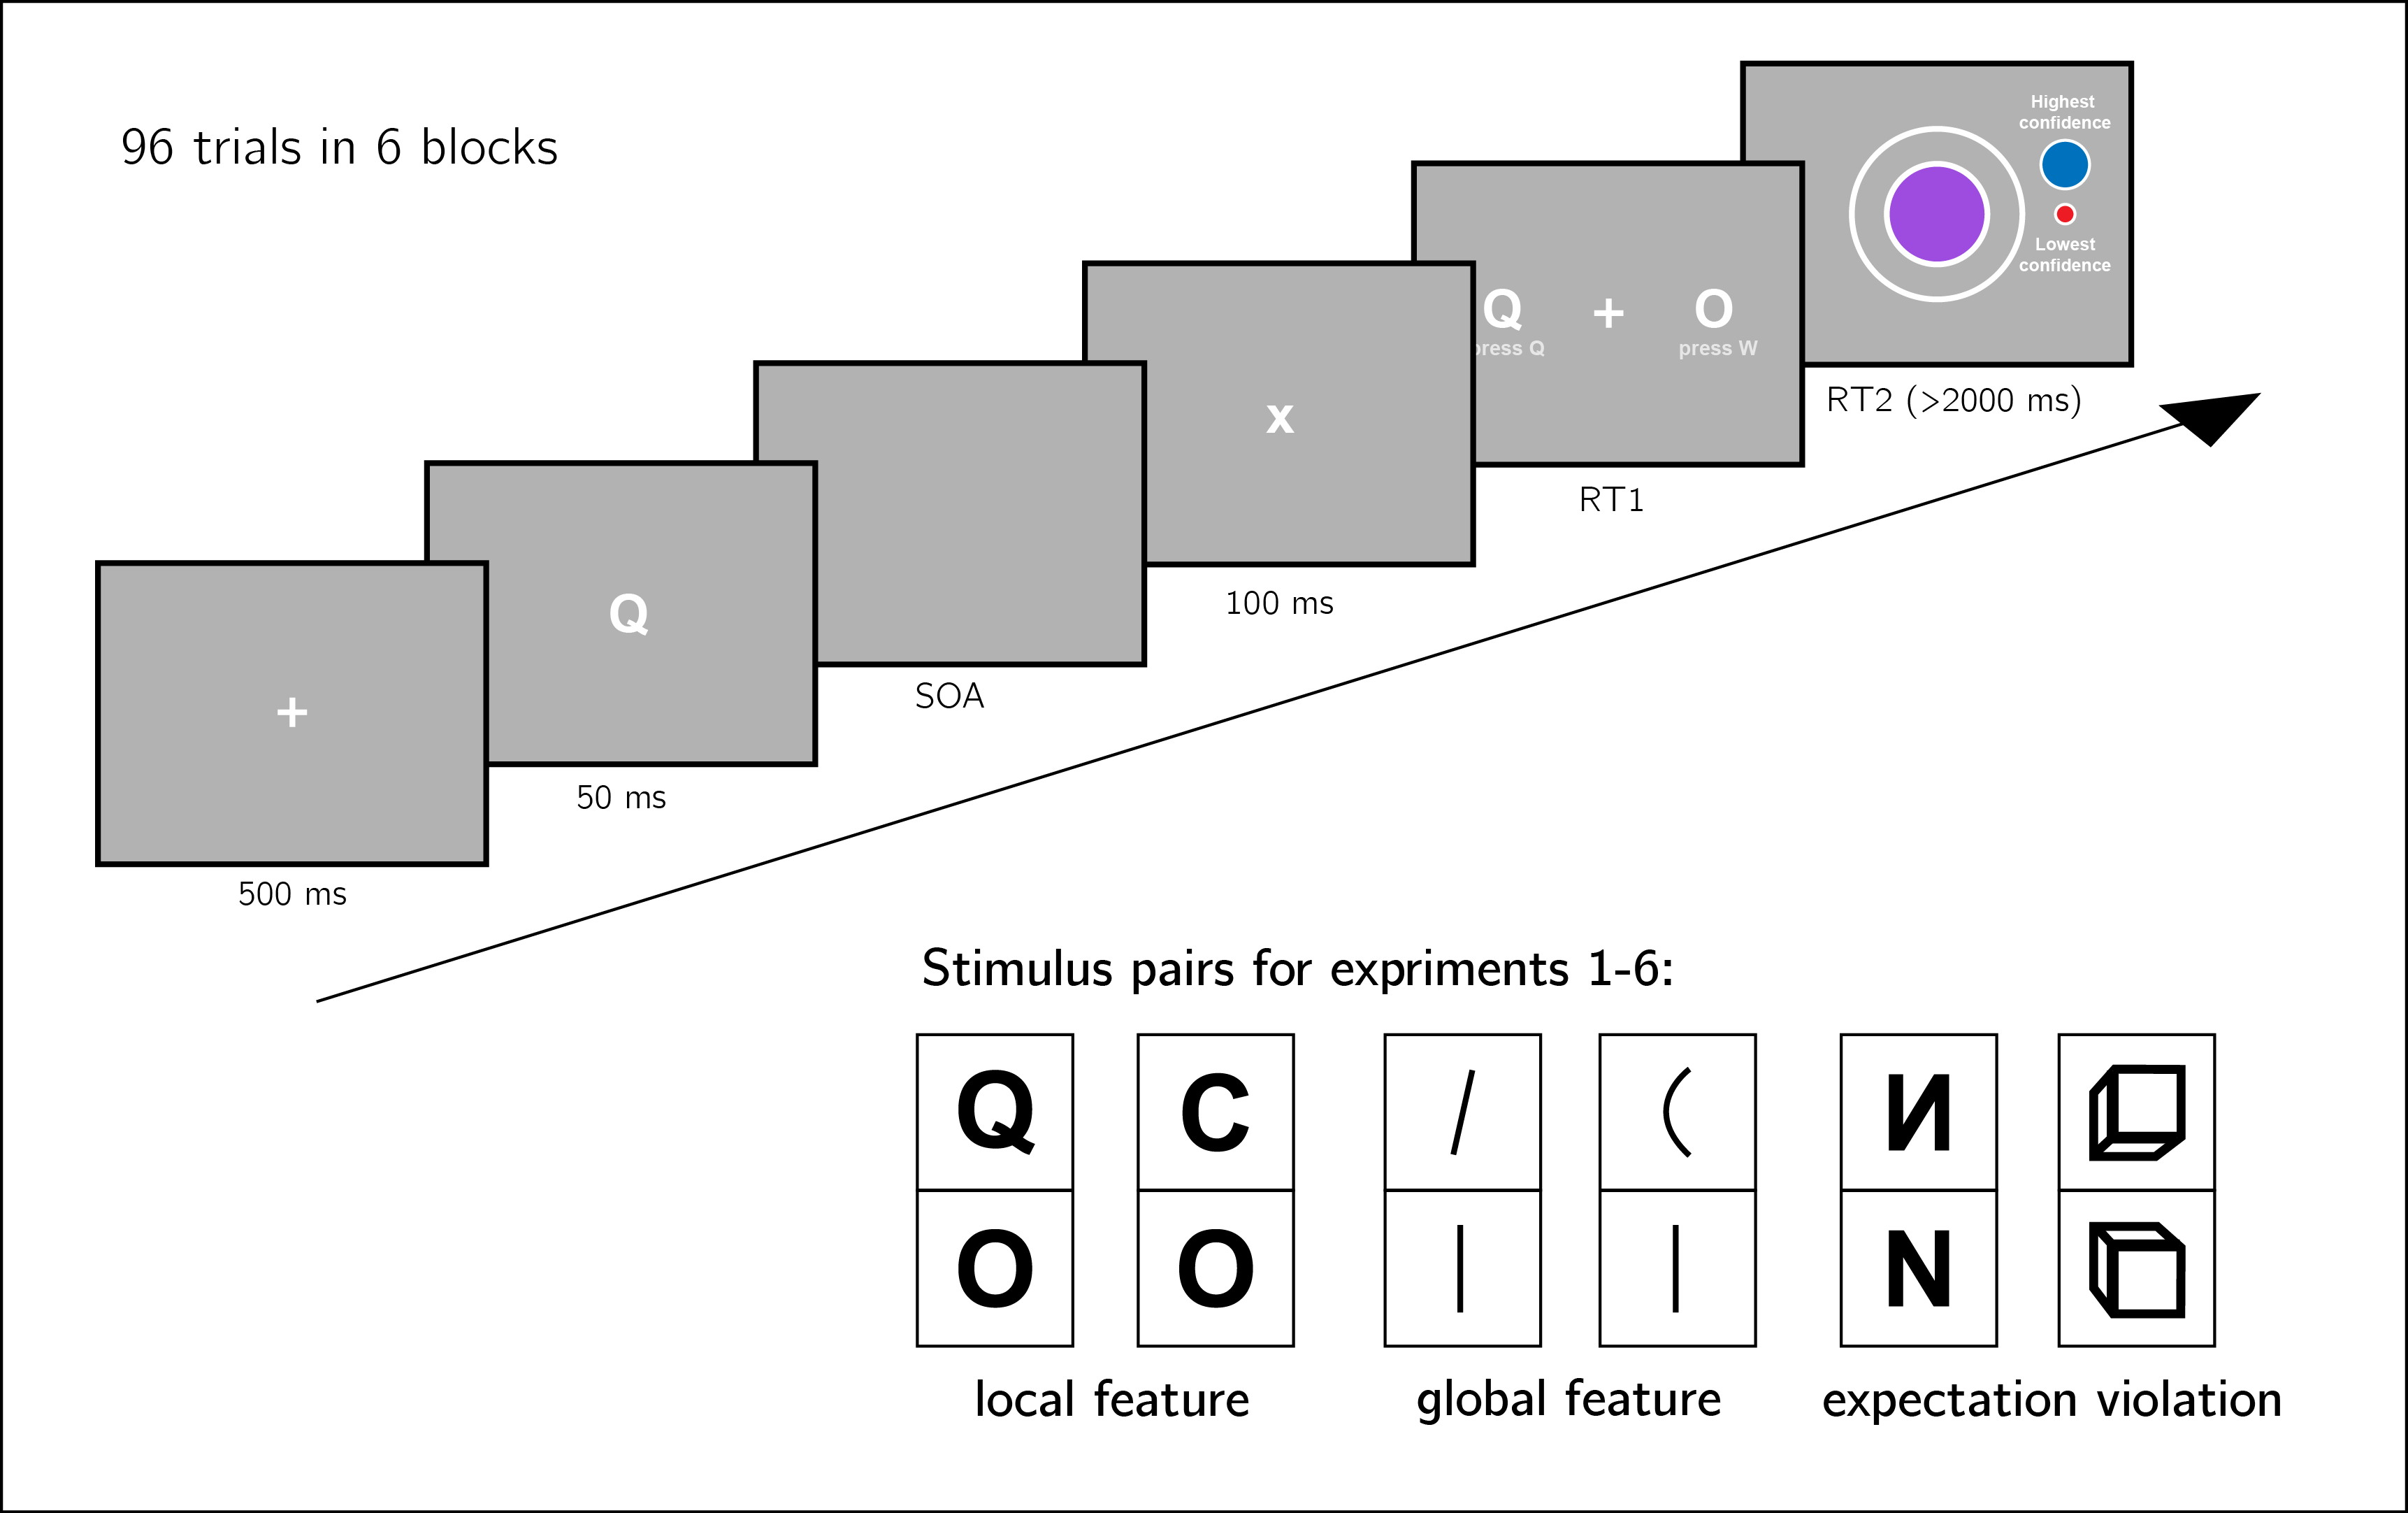
\includegraphics[width=1\linewidth]{figures/trial_structure_noVS} \caption{Experiment design. Metacognitive asymmetry effects will be tested for six stimulus features in six separate experiments, ecompassing three levels of abstraction: local features, global features, and expectation violations. The presented trial corresponds to the first stimulus pair, were *Q* and *O* are used as stimuli.}\label{fig:trialstructure}
\end{figure}

\hypertarget{randomization}{%
\subsubsection{Randomization}\label{randomization}}

The order and timing of experimental events will be determined pseudo-randomly by the Mersenne Twister pseudorandom number generator, initialized in a way that ensures registration time-locking (Mazor, Mazor, \& Mukamel, 2019).

\hypertarget{data-analysis}{%
\subsection{Data analysis}\label{data-analysis}}

We will use R (Version 3.6.0; R Core Team, 2019) and the R-packages \emph{BayesFactor} (Version 0.9.12.4.2; Morey \& Rouder, 2018), \emph{brms} (Version 2.13.0; Bürkner, 2018), \emph{broom} (Version 0.5.6; Robinson \& Hayes, 2020), \emph{cowplot} (Version 1.0.0; Wilke, 2019), \emph{dplyr} (Version 1.0.0; Wickham et al., 2020), \emph{ggplot2} (Version 3.3.1; Wickham, 2016), \emph{papaja} (Version 0.1.0.9942; Aust \& Barth, 2020), and \emph{tidyr} (Version 1.1.0; Wickham \& Henry, 2020) for all our analyses.

For each of the six stimulus pairs {[}\(S_1\), \(S_2\){]}, will test the following hypotheses:

\begin{enumerate}
\def\labelenumi{\arabic{enumi}.}
\tightlist
\item
  \textbf{Hypothesis 1}: Subjective confidence is higher for \(S_1\) responses than for \(S_2\) responses.
\end{enumerate}

For each of the six stimulus pairs, we will test the null hypothesis that subjective confidence for \(S_1\) responses is equal to or lower than subjective confidence for the feature-absent stimulus (\(H_o=conf_{S_1}\leq Conf_{S_2}\)).

\begin{enumerate}
\def\labelenumi{\arabic{enumi}.}
\setcounter{enumi}{1}
\tightlist
\item
  \textbf{Hypothesis 2}: Metacognitive sensitivity, measured as the area under the response conditional ROC curves, is higher for \(S_1\) responses than for \(S_2\) responses.
\end{enumerate}

For each of the six stimulus pairs, we will test the null hypothesis that metacognitive sensitivity for \(S_1\) responses is equal to or lower than metacognitive sensitivity for the \(S_2\) responses (\(H_o=auROC_{S_1}\leq auROC_{S_2}\)).

\begin{enumerate}
\def\labelenumi{\arabic{enumi}.}
\setcounter{enumi}{2}
\tightlist
\item
  \textbf{Hypothesis 3}: \(S_1\) responses are faster on average than \(S_2\) responses.
\end{enumerate}

For each of the six stimulus pairs, we will test the null hypothesis that log-transformed response times for \(S_1\) responses are equal to or higher than log-transformed resopnse times for \(S_2\) responses (\(H_o=log(RT_{S_1})\geq log(RT_{S_2})\)).

Hypotheses 1 and 2 correspond to the effects of stimulus type on metacognitive bias and metacognitive sensitivity, respectively. Although these two measures are theoretically independent, both bias and sensitivity are found to vary between detection \enquote{yes} and \enquote{no} responses. Hypothesis 3 is motivated by two observations from previous studies. First, detection \enquote{yes} responses are faster than detection \enquote{no} responses (Mazor et al., 2020). And second, when participants are not under strict time pressure, reaction time inversely scales with confidence (Calder-Travis, Charles, Bogacz, \& Yeung, 2020; Henmon, 1911; Pleskac \& Busemeyer, 2010). Based on these findings, if \(S_1\) and \(S_2\) responses are similar to detection \enquote{yes} and \enquote{no} responses not only in explicit confidence judgments, but also in response times, we should also expect a response time difference for these stimulus pairs.

\hypertarget{dependent-variables-and-analysis-plan}{%
\subsubsection{Dependent variables and analysis plan}\label{dependent-variables-and-analysis-plan}}

For the auROC analysis, confidence ratings will be divided into 20 bins. Response conditional ROC curves will be extracted by plotting the empirical cumulative distribution of confidence ratings for correct responses against the same cumulative distribution for incorrect responses. This will be done separately for the two responses \(S_1\) and \(S_2\), resulting in two curves. The area under the response-conditional ROC curve is a measure of metacognitive sensitivity (Fleming \& Lau, 2014). The difference between the areas for the two responses is a measure of metacognitive asymmetry (Meuwese et al., 2014). This difference will be used to test Hypothesis 2.

For each of the six experiments, all three hypotheses will be tested using a one tailed t-test at the group level with \(\alpha=0.05\).

In case of a null result, a Bayes factor will be computed using the BayesFactor R package (Morey, Rouder, Jamil, \& Morey, 2015) and using a Jeffrey-Zellner-Siow Prior with a medium rscale parameter of \(\sqrt{2}/2\).

\hypertarget{statistical-power}{%
\subsubsection{Statistical power}\label{statistical-power}}

Statistical power calculations were performed using the R-pwr package (Champely, 2020).

\begin{enumerate}
\def\labelenumi{\arabic{enumi}.}
\item
  Hypothesis 1 (MEAN CONFIDENCE): With 100 participants, we will have a statistical power of 95\% to detect effects of size 0.33, which is less than the standardized effect size we observed for confidence in our pilot sample (\(d=0.66\)).
\item
  Hypothesis 2 (METACOGNITIVE ASYMMETRY): With 100 participants, we will have a statistical power of 95\% to detect effects of size 0.33, which is less than the standardized effect size we observed for metacognitive sensitivity in our pilot sample (\(d=0.62\)).
\item
  Hypothesis 3 (RESPONSE TIME): With 100 participants, we will have a statistical power of 95\% to detect effects of size 0.33, which is less than the standardized effect size we observed for response time in our pilot sample (\(d=0.61\)).
\end{enumerate}

\hypertarget{rejection-criteria}{%
\subsubsection{Rejection criteria}\label{rejection-criteria}}

Participants will be excluded for performing below 60\% accuracy, for having extremely fast or slow reaction times in one or more of the tasks (below 250 milliseconds or above 5 seconds in more than 25\% of the trials), and for failing the comprehension check. Finally, for type-2 ROC curves to be generated, some responses must be incorrect. Thus, only participants who committed at least two errors of each error type (for example, mistaking a \emph{Q} of \emph{O} and mistaking an \emph{O} for \emph{Q}), will be included.

Trials with response time below 250 milliseconds or above 5 seconds will be excluded.

\hypertarget{data-availability}{%
\subsection{Data availability}\label{data-availability}}

All raw data will be made fully available on OSF and on the study's GitHub respository: \url{https://github.com/matanmazor/asymmetry}.
Pilot data is available at: \url{https://github.com/matanmazor/asymmetry/blob/master/Experiments/Q_in_O/results/pilot/jatos_results_batch3.csv}

\hypertarget{code-availability}{%
\subsection{Code availability}\label{code-availability}}

All analysis code will be openly shared on the study's GitHub repository: \url{https://github.com/matanmazor/asymmetry}. For complete reproducibility, the RMarkdown file used to generate the final version of the manuscript, including the generation of all figures and extraction of all test statistics, will be available on our GitHub repository.

\hypertarget{competing-interests}{%
\subsection{Competing interests}\label{competing-interests}}

The authors declare no competing interests.

\newpage

\hypertarget{references}{%
\section{References}\label{references}}

\begingroup
\setlength{\parindent}{-0.5in}
\setlength{\leftskip}{0.5in}

\hypertarget{refs}{}
\leavevmode\hypertarget{ref-R-papaja}{}%
Aust, F., \& Barth, M. (2020). \emph{papaja: Create APA manuscripts with R Markdown}. Retrieved from \url{https://github.com/crsh/papaja}

\leavevmode\hypertarget{ref-R-brms_b}{}%
Bürkner, P.-C. (2018). Advanced Bayesian multilevel modeling with the R package brms. \emph{The R Journal}, \emph{10}(1), 395--411. \url{https://doi.org/10.32614/RJ-2018-017}

\leavevmode\hypertarget{ref-calder2020bayesian}{}%
Calder-Travis, J., Charles, L., Bogacz, R., \& Yeung, N. (2020). Bayesian confidence in optimal decisions.

\leavevmode\hypertarget{ref-R-pwr}{}%
Champely, S. (2020). \emph{Pwr: Basic functions for power analysis}. Retrieved from \url{https://CRAN.R-project.org/package=pwr}

\leavevmode\hypertarget{ref-coldren2000asymmetries}{}%
Coldren, J. T., \& Haaf, R. A. (2000). Asymmetries in infants' attention to the presence or absence of features. \emph{The Journal of Genetic Psychology}, \emph{161}(4), 420--434.

\leavevmode\hypertarget{ref-de1988knowing}{}%
De Cornulier, B. (1988). Knowing whether, knowing who, and epistemic closure. \emph{Questions and Questioning}, 182--192.

\leavevmode\hypertarget{ref-de2015jspsych}{}%
De Leeuw, J. R. (2015). JsPsych: A javascript library for creating behavioral experiments in a web browser. \emph{Behavior Research Methods}, \emph{47}(1), 1--12.

\leavevmode\hypertarget{ref-fleming2014measure}{}%
Fleming, S. M., \& Lau, H. C. (2014). How to measure metacognition. \emph{Frontiers in Human Neuroscience}, \emph{8}, 443.

\leavevmode\hypertarget{ref-frith1974acurious}{}%
Frith, U. (1974). Acurious effect with reversed letters explained by a theory of schema. \emph{Perception \& Psychophysics}, \emph{16}(1), 113--116.

\leavevmode\hypertarget{ref-gandolfo2020asymmetric}{}%
Gandolfo, M., \& Downing, P. E. (2020). Asymmetric visual representation of sex from human body shape. \emph{Cognition}, \emph{205}, 104436.

\leavevmode\hypertarget{ref-hearst1991psychology}{}%
Hearst, E. (1991). Psychology and nothing. \emph{American Scientist}, \emph{79}(5), 432--443.

\leavevmode\hypertarget{ref-henmon1911relation}{}%
Henmon, V. A. C. (1911). The relation of the time of a judgment to its accuracy. \emph{Psychological Review}, \emph{18}(3), 186.

\leavevmode\hypertarget{ref-higham2009investigating}{}%
Higham, P. A., Perfect, T. J., \& Bruno, D. (2009). Investigating strength and frequency effects in recognition memory using type-2 signal detection theory. \emph{Journal of Experimental Psychology: Learning, Memory, and Cognition}, \emph{35}(1), 57.

\leavevmode\hypertarget{ref-kanai2010subjective}{}%
Kanai, R., Walsh, V., \& Tseng, C.-h. (2010). Subjective discriminability of invisibility: A framework for distinguishing perceptual and attentional failures of awareness. \emph{Consciousness and Cognition}, \emph{19}(4), 1045--1057.

\leavevmode\hypertarget{ref-kellij2018foundations}{}%
Kellij, S., Fahrenfort, J., Lau, H., Peters, M. A., \& Odegaard, B. (2018). The foundations of introspective access: How the relative precision of target encoding influences metacognitive performance.

\leavevmode\hypertarget{ref-lange2015just}{}%
Lange, K., Kühn, S., \& Filevich, E. (2015). " Just another tool for online studies''(JATOS): An easy solution for setup and management of web servers supporting online studies. \emph{PloS One}, \emph{10}(6), e0130834.

\leavevmode\hypertarget{ref-levitt1971transformed}{}%
Levitt, H. (1971). Transformed up-down methods in psychoacoustics. \emph{The Journal of the Acoustical Society of America}, \emph{49}(2B), 467--477.

\leavevmode\hypertarget{ref-mazor2020distinct}{}%
Mazor, M., Friston, K. J., \& Fleming, S. M. (2020). Distinct neural contributions to metacognition for detecting, but not discriminating visual stimuli. \emph{Elife}, \emph{9}, e53900.

\leavevmode\hypertarget{ref-mazor2019novel}{}%
Mazor, M., Mazor, N., \& Mukamel, R. (2019). A novel tool for time-locking study plans to results. \emph{European Journal of Neuroscience}, \emph{49}(9), 1149--1156.

\leavevmode\hypertarget{ref-mccarthy2015p5}{}%
McCarthy, L. (2015). P5. Js. \emph{URL: Https://P5js. Org}, \emph{3}.

\leavevmode\hypertarget{ref-meuwese2014subjective}{}%
Meuwese, J. D., Loon, A. M. van, Lamme, V. A., \& Fahrenfort, J. J. (2014). The subjective experience of object recognition: Comparing metacognition for object detection and object categorization. \emph{Attention, Perception, \& Psychophysics}, \emph{76}(4), 1057--1068.

\leavevmode\hypertarget{ref-R-BayesFactor}{}%
Morey, R. D., \& Rouder, J. N. (2018). \emph{BayesFactor: Computation of bayes factors for common designs}. Retrieved from \url{https://CRAN.R-project.org/package=BayesFactor}

\leavevmode\hypertarget{ref-morey2015package}{}%
Morey, R. D., Rouder, J. N., Jamil, T., \& Morey, M. R. D. (2015). Package ``bayesfactor''. \emph{URLh Http://Cran/R-Projectorg/Web/Packages/BayesFactor/BayesFactor Pdf I (Accessed 1006 15)}.

\leavevmode\hypertarget{ref-newman1980feature}{}%
Newman, J. P., Wolff, W. T., \& Hearst, E. (1980). The feature-positive effect in adult human subjects. \emph{Journal of Experimental Psychology: Human Learning and Memory}, \emph{6}(5), 630.

\leavevmode\hypertarget{ref-oaksford2002contrast}{}%
Oaksford, M. (2002). Contrast classes and matching bias as explanations of the effects of negation on conditional reasoning. \emph{Thinking \& Reasoning}, \emph{8}(2), 135--151.

\leavevmode\hypertarget{ref-oaksford2001probabilistic}{}%
Oaksford, M., \& Chater, N. (2001). The probabilistic approach to human reasoning. \emph{Trends in Cognitive Sciences}, \emph{5}(8), 349--357.

\leavevmode\hypertarget{ref-pleskac2010two}{}%
Pleskac, T. J., \& Busemeyer, J. R. (2010). Two-stage dynamic signal detection: A theory of choice, decision time, and confidence. \emph{Psychological Review}, \emph{117}(3), 864.

\leavevmode\hypertarget{ref-R-base}{}%
R Core Team. (2019). \emph{R: A language and environment for statistical computing}. Vienna, Austria: R Foundation for Statistical Computing. Retrieved from \url{https://www.R-project.org/}

\leavevmode\hypertarget{ref-R-broom}{}%
Robinson, D., \& Hayes, A. (2020). \emph{Broom: Convert statistical analysis objects into tidy tibbles}. Retrieved from \url{https://CRAN.R-project.org/package=broom}

\leavevmode\hypertarget{ref-sainsbury1971feature}{}%
Sainsbury, R. (1971). The ``feature positive effect'' and simultaneous discrimination learning. \emph{Journal of Experimental Child Psychology}, \emph{11}(3), 347--356.

\leavevmode\hypertarget{ref-takeda2000inhibitory}{}%
Takeda, Y., \& Yagi, A. (2000). Inhibitory tagging in visual search can be found if search stimuli remain visible. \emph{Perception \& Psychophysics}, \emph{62}(5), 927--934.

\leavevmode\hypertarget{ref-treisman1988feature}{}%
Treisman, A., \& Gormican, S. (1988). Feature analysis in early vision: Evidence from search asymmetries. \emph{Psychological Review}, \emph{95}(1), 15.

\leavevmode\hypertarget{ref-treisman1985search}{}%
Treisman, A., \& Souther, J. (1985). Search asymmetry: A diagnostic for preattentive processing of separable features. \emph{Journal of Experimental Psychology: General}, \emph{114}(3), 285.

\leavevmode\hypertarget{ref-von1994visual}{}%
Von Grünau, M., \& Dubé, S. (1994). Visual search asymmetry for viewing direction. \emph{Perception \& Psychophysics}, \emph{56}(2), 211--220.

\leavevmode\hypertarget{ref-walton1992nonfallacious}{}%
Walton, D. (1992). Nonfallacious arguments from ignorance. \emph{American Philosophical Quarterly}, \emph{29}(4), 381--387.

\leavevmode\hypertarget{ref-wang1994familiarity}{}%
Wang, Q., Cavanagh, P., \& Green, M. (1994). Familiarity and pop-out in visual search. \emph{Perception \& Psychophysics}, \emph{56}(5), 495--500.

\leavevmode\hypertarget{ref-R-ggplot2}{}%
Wickham, H. (2016). \emph{Ggplot2: Elegant graphics for data analysis}. Springer-Verlag New York. Retrieved from \url{https://ggplot2.tidyverse.org}

\leavevmode\hypertarget{ref-R-dplyr}{}%
Wickham, H., François, R., Henry, L., \& Müller, K. (2020). \emph{Dplyr: A grammar of data manipulation}. Retrieved from \url{https://CRAN.R-project.org/package=dplyr}

\leavevmode\hypertarget{ref-R-tidyr}{}%
Wickham, H., \& Henry, L. (2020). \emph{Tidyr: Tidy messy data}. Retrieved from \url{https://CRAN.R-project.org/package=tidyr}

\leavevmode\hypertarget{ref-R-cowplot}{}%
Wilke, C. O. (2019). \emph{Cowplot: Streamlined plot theme and plot annotations for 'ggplot2'}. Retrieved from \url{https://CRAN.R-project.org/package=cowplot}

\endgroup

\newpage

\hypertarget{supplementary-information}{%
\section{Supplementary information}\label{supplementary-information}}

\hypertarget{pilot-data-and-analysis}{%
\section{Pilot data and analysis}\label{pilot-data-and-analysis}}

\hypertarget{pilot-experiment}{%
\subsection{Pilot Experiment}\label{pilot-experiment}}

30 participants were recruited from Prolific for our pilot experiment. We followed a similar procedure to the one described in the Methods section, using \emph{Q} and \emph{O} as our stimuli. In this pilot study we also replicated the visual-search asymmetry for these stimuli. To keep the experiment short and participants engaged, participants only completed 32 discrimination trials. The experiment took about 13.5 minutes to complete. Subjects were paid £1.25 for their participation.

Mean accuracy was 0.80 in the discrimination task, 0.96 in the Q-in-O search task, and 0.95 in the O-in-Q search task. We excluded participants for performing below 70\% accuracy in one or two of the search tasks, for performing below 60\% accuracy in the discrimination task, for having extremely fast or slow reaction times in one or more of the tasks (below 250 milliseconds or above 5 seconds in more than 25\% of the trials), and for failing the comprehension check. Overall we excluded 0 participants, leaving 30 participants for the main analysis.

\hypertarget{visual-search-task-search-asymmetry-replication}{%
\subsection{Visual search task: search asymmetry replication}\label{visual-search-task-search-asymmetry-replication}}

Search time analysis was performed on correct trials with reaction time between 250 and 5000 milliseconds. Search slopes for the response time/set size function were extracted for each participant, task and response, and then subjected to a two-way analysis of variance. As expected, we observed significant effects for target identity (mean search slope for \emph{Q-in-O} search: 18.93 ms/item; mean search slope for \emph{O-in-Q} search: 54.89 ms/item; \(F(1, 116) = 44.39\), \(\mathit{MSE} = 873.80\), \(p < .001\)) and response (mean search slope for target absent responses: 48.04; mean search slope for target present responses: 25.78; \(F(1, 116) = 17.01\), \(\mathit{MSE} = 873.80\), \(p < .001\); see Figure \ref{fig:RT-pilot}). An interaction effect was also significant (\(F(1, 116) = 8.91\), \(\mathit{MSE} = 873.80\), \(p = .003\)). These results match previous reports of steeper search slopes for searching a circle among circles crossed by a line than for the inverse search (e.g., Treisman \& Souther, 1985).

\begin{figure}
\centering
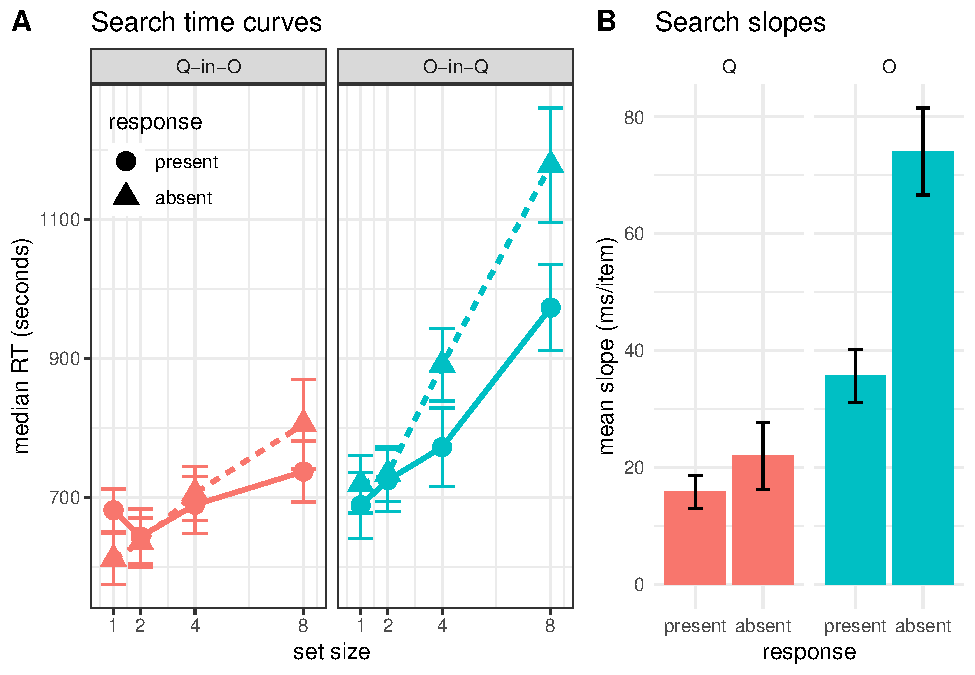
\includegraphics{asymmetry_files/figure-latex/RT-pilot-1.pdf}
\caption{\label{fig:RT-pilot}A: Median search time by distractor set size for the two search tasks and two responses. Correct responses only. Error bars represent the standard error of the median. B: mean search slope per target (Q or O) and response (present or absent). Error bars represent the standard error of the mean.}
\end{figure}

\hypertarget{discrimination-task-metacognitive-asymmetry}{%
\subsection{Discrimination task: metacognitive asymmetry}\label{discrimination-task-metacognitive-asymmetry}}

Mean accuracy in the discrimination task was 0.81 (\(M = 0.81\), 95\% CI \([0.77\), \(0.84]\)). Participants showed no consistent bias in their responses (\(M = 0.53\), 95\% CI \([0.48\), \(0.57]\)). On a scale of 0 to 1, mean confidence level was 0.56 (\(M = 0.56\), 95\% CI \([0.47\), \(0.64]\)). Confidence was higher for correct than for incorrect responses (\(M_d = 0.15\), 95\% CI \([0.09\), \(0.21]\), \(t(29) = 5.24\), \(p < .001\)).

\emph{Hypothesis 1}: In line with our hypothesis, confidence was generally higher for \emph{Q} (feature present) responses than for \emph{O} (feature absent) responses (\(M_d = 0.10\), 95\% CI \([0.05\), \(0.16]\), \(t(29) = 3.63\), \(p = .001\); cohen's d = 0.66).

\emph{Hypothesis 2}: In order to measure metacognitive asymmetry, we extracted the response-conditional type-2 ROC (rc-ROC) curves for the two responses (\emph{Q} and \emph{O}) in the discrimination task. This was done by plotting the cumulative distribution of confidence ratings (high to low) for correct responses against the same distribution for incorrect responses. The area under the rc-ROC curve (auROC) was then taken as a measure of metacognitive sensitivity (Kanai et al., 2010; Meuwese et al., 2014). In line with our hypothesis, auAUC for \emph{Q} responses (\(M = 0.69\), 95\% CI \([0.61\), \(0.77]\)) was marginally higher than for \emph{O} responses (\(M = 0.61\), 95\% CI \([0.54\), \(0.68]\); \(t(11) = 2.16\), \(p = .054\); Cohen's d = 0.62; see Figure \ref{fig:rc-ROC-pilot}), mirroring the metacognitive asymmetry for detection judgments.

\emph{Hypothesis 3}: In line with our hypothesis, \emph{Q} responses were faster on average than \emph{O} responses (\(t(29) = -3.32\), \(p = .002\) ; Cohen's d =
0.61).

\begin{figure}
\centering
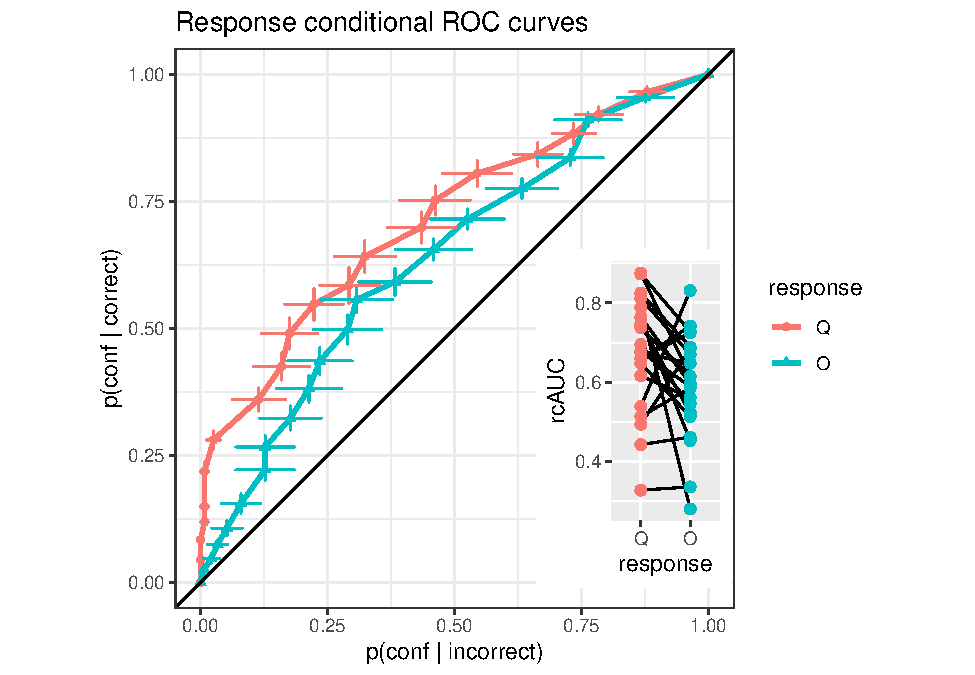
\includegraphics{asymmetry_files/figure-latex/rc-ROC-pilot-1.pdf}
\caption{\label{fig:rc-ROC-pilot}response conditional ROC curves for the two discrimination responses. The area under the curve is a measure of metacognitive sensitivity. Bottom right inset: distributions of the area under the curve for the two responses, across participants. Overall, participants had lower metacognitive insight into the accuracy of their \enquote{O} responses.}
\end{figure}

\end{document}
